\documentclass[12pt]{article}

\usepackage{fullpage,url,amssymb,epsfig,color,pdfpages,xspace,enumerate,multirow,enumitem,graphicx,amsmath}
\usepackage{listings}
\usepackage[pdftitle={ECE457b Project},%
pdfsubject={University of Waterloo, ECE 457b, Winter 2017},%
pdfauthor={Daniel Cardoza, Lara Janecka, Hong Wang}]{hyperref}

\begin{document}

\begin{center}
{\Large\bf Report for}\\
\vspace{1mm}
{\Large\bf ECE457B Course Project, Winter 2017}\\
\vspace{2mm}
{\Large\bf Title\_Of\_Project}\\
\vspace{4mm}
{Daniel Cardoza/dpmcardo/20471664}\\
{Lara Janecka/lajaneck/20460089}\\
{Hong Wang/hmwang/20469058}\\
\vspace{2mm}
\textbf{Due Date: April 3, 2017}
\end{center}

\definecolor{care}{rgb}{0,0,0}
\def\question#1{\item[\bf #1.]}
\def\part#1{\item[\bf #1)]}
\newcommand{\pc}[1]{\mbox{\textbf{#1}}} % pseudocode

\section{Abstract}

\section{Introduction}

\section{Background}
\subsection{Music Files}
The files used for analysis were primarily wav files. To use another type of file required conversion into a wav file. Wav files consist of a header containing relevant information such as sample rate and the number of channels, and the sound data for each sample. This format does not compress the data and thus was chosen of the most accurate results. A parser was written to extract the sample rate and a waveform for the sound data. The sample rate is the number of samples taken per second. For CD quality (the most common type of file looked at) this value is 44,100. The waveform is the list of data for the sound data at each sample point for each channel.

\subsection{Stepmania Files}
\subsection{Overview}

Stepmania is a cross-platform dance and rhythm game. Players select a song and corresponding leve of difficulty when playing. Then, players view a screen where up, down, left and right arrows rise up on the screen. When the arrow reaches a certain point, the user clicks the corresponding arrow key on their keyboard.\\

Stepmania uses custom files containing necessary metadata and audio information. In the context of this project, each stepmania arrow corresponds to a different beat in the song being played. This makes the gaming experience more natural and enjoyable for the player. Our project seeks to perform beat detection, and then generate the corresponding Stepmania file with beats at the discrete times we detect. Note that a Stepmania file may only have steps for a subset of the beats in a song.\\

\subsection{File Format}

The Stepmania file format contains necessary header information indicating the corresponding song for the file as well as information about the song itself and the file creator. The specific part of the song detailing the steps of the corresponding is in the \textbf{NOTES} section. Each notes is composed of measures, where different steps in a measure are separated by the same unit of time. Each line consists of 4 integers where each digit represents a different arrow. For example the line \textbf{1001} indicates that for this step, the left and right arrow characters on a keyboard should be clicked.\\

An example of this beat information in the Stepmania file can be seen below:\\
\begin{lstlisting}
#NOTES:
     these are some sample steps:
     5:
     0.000,0.250,0.500,0.750,1.000: // 5 measures
// measure 1
2010
0000
0100
0000
, // measure 2
...
\end{lstlisting}

In the context of our project, we seek to detect beats for a given song and generate a step file from this information. As well, since Stepmania files don't have a step for each beat, we implement a heuristic function that predicts if a beat is a step based on the time of the last step and the amount of beats that has occurred since the last step.\\




\subsection{Beat Detection}
Notes:
	\begin{itemize}
		\item humans have temporal masking of about 3ms
		\item humans hear frequency range of 20-20000Hz
		\item humans have frequency accuracy to 3.6Hz
		\item music contains sounds from 100-3200Hz (most often)
	\end{itemize}


\section{Solution}

\subsection{Feature Extraction}
Three kinds of features were used in the scope of this project. There were many other potentially useful features that could be extracted from audio files for use in beat detection, but many of them required complex audio processing beyond the knowledge of the authors of this report. This project focused on power variance, bandwidth power variance, and change in peak frequency. To accommodate for audio temporal masking in human hearing the sample rate was decreased to a sample every three milliseconds. This was done by aggregating samples into a chunk and comparing that with the other aggregated samples in its neighborhood. A chunk of data is the number of samples calculated to span three milliseconds of time.

\begin{align*}
	\text{chunk size} = c &= \frac{\text{number of samples}}{300}\\
\end{align*}

Each type of feature extraction generated data relative to the song it is in. This is due to the range of song genres considered in the scope of this project. Data comparisons using absolute values would confuse the training data when transitioning between songs, for example the electronic music has a much higher average frequency than dubstep. The solution to this was to compare features to a neighborhood of data to get relative values.

Since most songs go through various phases in which the pitch, tempo, and power levels can be drastically different the neighborhood of comparison was limited to one seconds worth of data. This value was chosen because it was small enough to capture the changes in features while still being large enough to contain data about the current state of the song. One second is also the unit used when describing the tempo of a song when making a rough estimate. This allowed for a benchmark of what would be a reasonable number of beats in a second when comparing to the genre of the song.

\subsubsection{Power Variance}
The waveform of a sound file represents its data as energy levels within a channel at a given sample. The total power level of a sample can be calculated by summing the square over all channels in the waveform.

\begin{align*}
 	\text{Power}(x) &= \sum_j^{channels} x[j]^2
 \end{align*}

Aggregation was done through averaging to lessen the number of samples being fed into the the network and to try to remove some of the noise within the signal.

\begin{align*}
	\text{Chunks}(x) &= \frac{\sum_{i=0}^{c}\text{Power}(x+i)}{c}
\end{align*}
The averaged power of a chunk is then compared to the average power of the surrounding second of data to account for different median power levels based on genre of song or mood at that moment within the song.

\begin{align*}
	\text{PowerVariance}[x] &= \text{Chunks}[x] - \frac{\sum_{i-150}^{i+150}\text{Chunks}[i]}{300}
\end{align*}

\subsubsection{Bandwidth Energy Variance}
The power level of a song ignores the frequency aspect of audio processing. The frequency of sounds within a song heavily influence the placement of beats and thus cannot be ignored. To account for this a feature was added that breaks a chunk into frequencies and sums the energy within set bandwidth ranges. These ranges were pulled from a paper written by Eric Scheirer in which he attempted to detect beats in music using only frequency analysis. In it he outlined 5 bandwidth ranges to group by, 0-200Hz, 200-400Hz, 400-800Hz, 800-1600Hz, and 1600-3200Hz. Frequencies over 3200Hz were ignored as their prevalence in music is limited due to discomfort caused to listeners.

First the energy across channels is calculated to account for multichannel songs.
\begin{align*}
 	\text{Energy}(x) &= \sum_j^{channels} x[j]
 \end{align*}

 The audio file is once again aggregated into chunks of roughly three milliseconds worth of data. The aggregation function is now a Discrete Fourier Transform. This was calculated using Python's SciPy library.

 \begin{align*}
 	F[i] =  \texttt{scipy.fft}(Energy[i \dots i+chunkSize])
 \end{align*}

The signals in F were divided into the above stated bandwidth ranges and their amplitudes summed. This represents the value of the cumulative power within each bandwidth range. These values were then compared to the surrounding second's worth of data using the same procedure as used when calculating the average power variance. This resulted in five values representing the power variance across the five bandwidth ranges for that chunk of data.

\subsubsection{Peak Frequency Change}
One of the biggest methods used by humans for identifying beats is to detect changes in the dominant frequency. This is used in the music genres aimed at dancing (the primary focus of this report was on such songs) to sync up crows by having frequent changes between a high pitched melody and a low pitched base line. An extreme example of this is a drop in typical dubstep songs. This feature most closely represents how humans intuitively detect beats.

The peak frequency for a chunk was found by calculating the energy for sample and taking the Fast Fourier Transform of each chunk using the same procedure as used when calculating the bandwidth energy variance. The peak frequency was found by finding the highest amplitude within the chunk in question's data and taking the frequency at which it occurred. This value itself means very little since different song genres and within the songs the median frequency varies greatly. Unlike previous features, comparing the peak frequency to the surrounding second's worth of data would make little sense since the peak frequency varies greatly within a second. Instead, the peak frequency is compared only to the next value. This aims to identify only the instance of a sudden drop to try to refine beat identification.

\subsection{Multilayer Perceptron}


\subsection{Dataset Construction and Format}

\subsubsection{Dataset Format}

In order to use a multilayer perceptron network, supervised learning must be used in order to let the network learn the function you are trying to represent or approximate. For our project, the network is trained on a set of timeframes corresponding to the wavelet file for an audio track in order to detect beats. A timeframe can be defined as a portion of the audio signal for a music file. Thus, a dataset that mapped different timeframes of an audio file to a beat was required. This required researching into datasets that exposed both the metadata information for a large corpus of  audio files, and the discrete times for when beats occur.\\

With the above requirements, we could define the necessary format of our dataset. Our dataset required pairs of files for an audio track : an uncompressed wavelet file in the ‘.wav’ format and a corresponding ‘.beats’ file containing comma separated times for when beats occurred in a song.\\

\subsubsection{Music Information Retrieval Evaluation Exchange (MIREX)}

Our initial dataset was a small dataset used for a 2012 audio beat tracking competition provided by the Music Information Retrieval Evaluation Exchange (MIREX). MIREX is a contest and conference organized by the graduate school of computer science at the University of Illinois Urbana-Champaign. It provides datasets for contests attempting to identify optimal algorithms for beat detection, tempo change detection and other audio analytics. \\

The dataset used consisted of 100 songs, where each song had a file containing the times when a human audience believe beats occurred. Each audio file was in the uncompressed wavelet format, with 1 audio channel and at a standard 44.1KHz sampling rate of timeframes per second. However each song in this dataset was less than 30 seconds in length, so it did not provide enough timeframes to train any neural network model. \\

\subsubsection{Million Song Dataset}

The Million Song Dataset is a dataset containing audio analysis features for millions of songs. One of the features analyzed and available, is the discrete timing of beats. This dataset is openly available and was produced by the Echo Nost, an audio analytics company. This dataset provided all of the necessary beats information for an incredibly large corpus of songs, 280GB in size. However, unlike the Mirex dataset, it did not provide any media files that would allow us to use as training inputs to our model. Thus, we had to implement our own solution.

\subsubsection{Google Play Music}

In order to build a corpus of media files, we used the GooglePlayMusic API to to download songs. For each song we found in a subset of the MillionSongDataset, we extracted its track title, downloaded the audio file in the MPEG-2 format (mp3), and then converted it to the uncompressed wavelet format. This conversion was performed using the popular FFMPEG utility. 
\begin{center}
	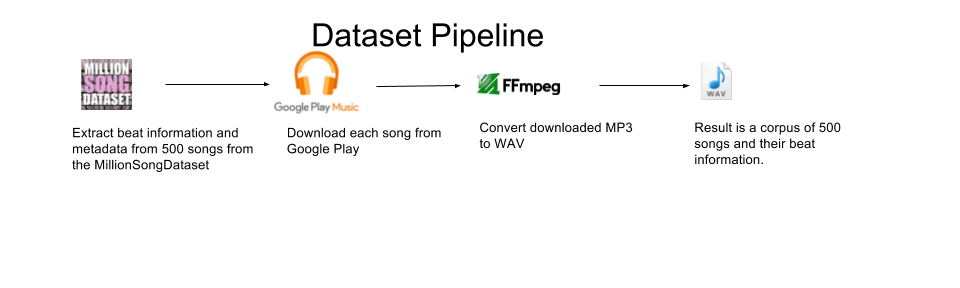
\includegraphics[scale=0.55]{dataset_flow.png}
\end{center}

\section{Results}

\subsection{Method of Evaluation}

\subsection{Accuracy}

\subsection{Potential Sources of Errors}

\subsubsection{Feature Extraction}

\subsubsection{Network Values}

\section{Conclusion}

\subsection{Future Improvements}

\subsubsection{Feature Extraction}

\subsubsection{Recurrent Networks}


\section{References}

\end{document}
